\documentclass[11pt,xcolor=dvipsnames]{beamer}
\usetheme{Warsaw}

\PassOptionsToPackage{table,svgnames,dvipsnames}{xcolor}

\usepackage[utf8]{inputenc}\usepackage{amsmath}
\usepackage{amsfonts}
\usepackage{amssymb}
\usepackage{graphicx}
\usepackage{grffile}
\usepackage{tikz}
\usetikzlibrary{graphs,graphs.standard}
\usepackage{multicol}
\usetikzlibrary{arrows,positioning}
\usepackage{multicol}
\usepackage{makecell}
\usepackage{pbox}
\usepackage{appendixnumberbeamer}
\usepackage{subfig}
\usepackage{tikz-cd}
\usepackage{algorithm}
\usepackage[noend]{algpseudocode}
\usepackage[pdf]{graphviz}

\DeclareMathOperator*{\argmax}{arg\,max}
\DeclareMathOperator*{\argmin}{arg\,min}
\DeclareMathOperator{\Tr}{Tr}

\author[Jan Schopohl, Dominik Fuchsgruber]{Jan Schopohl, Dominik Fuchsgruber \\[10mm]{\small Supervisor: Maxim Maximov}}
\title{Variational Style Transfer}
\date{December 3rd, 2019}

\institute{Department of Informatics, Technical University of Munich}
%\setbeamercovered{transparent} 
%\setbeamertemplate{navigation symbols}{} 
%\logo{} 
%\institute{} 
%\date{} 
%\subject{} 

\setbeamertemplate{sidebar right}{}
\setbeamertemplate{footline}{%
\hfill\usebeamertemplate***{navigation symbols}
\hspace{1cm}\insertframenumber{}/\inserttotalframenumber}

    \setbeamertemplate{headline}{}
    
   
\usepackage[backend=bibtex]{biblatex}
\addbibresource{presentation.bib}
        
\begin{document}

\begin{frame}
\titlepage
\end{frame}



\begin{frame}
	
\frametitle{Artistic Style Transfer}


\begin{multicols*}{2}
\begin{large}
Given a \textcolor{blue}{\textbf{content image} $C$} and an artistic \textcolor{Plum}{\textbf{style image $S$}}: 


\vspace{20pt}

$\rightarrow$ \textbf{Stylization}: Image with content similar to \textcolor{blue}{\textbf{$C$}} and a style similar to \textcolor{Plum}{\textbf{$S$}} 

\vspace{40pt}

How to combine \textcolor{red}{\textbf{different styles}}?
\end{large}

\begin{figure}
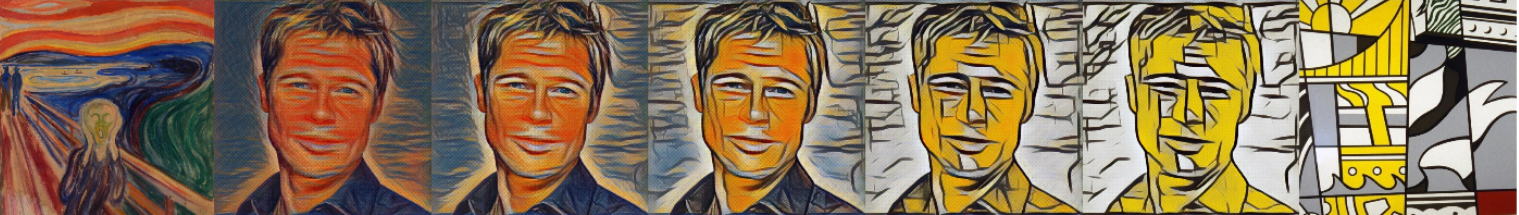
\includegraphics[scale=0.2]{interpolation.png}
\end{figure}

\columnbreak

\begin{figure}
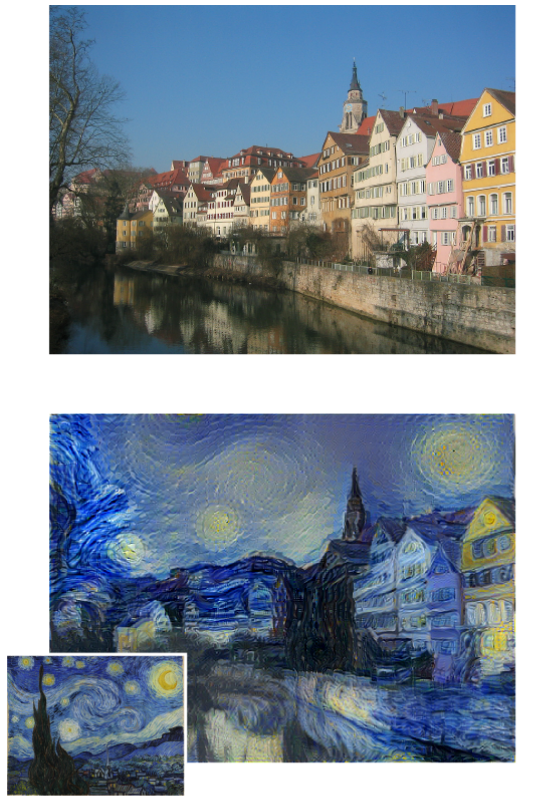
\includegraphics[scale=0.2]{styletransfergatysetal.png}
\end{figure}

\end{multicols*}
\end{frame}

\begin{frame}
\frametitle{Related Work}

\begin{itemize}
	\item \textcolor{gray}{\cite{gatys}}: Optimize random image to fit \textcolor{blue}{\textbf{$C$}} content-wise and \textcolor{Plum}{\textbf{$S$}} style-wise $\rightarrow$ \textbf{\textcolor{red}{very slow!}}
	\vspace{10pt}
	
	\item \textcolor{gray}{\cite{adain}}: \textbf{Autoencoders} to encode \textcolor{blue}{\textbf{$C$}} and \textcolor{Plum}{\textbf{$S$}}, use Adaptive Instance Normalization (\textbf{AdaIn}) to transfer the style
	\vspace{10pt}
	
	\item \textcolor{gray}{\cite{disentanglement}}: Separate Encoders for \textcolor{blue}{\textbf{content}} and \textcolor{Plum}{\textbf{style}} \\ $\rightarrow$ \textcolor{red}{\textbf{Disentanglement}}
	\vspace{10pt}
	
	\item \textcolor{gray}{\cite{vae}}: \textbf{Variational Autoencoders} encode into a \textbf{smooth latent space} \\
	$\rightarrow$ Good for \textcolor{red}{\textbf{interpolation between encodings}}
	\vspace{10pt}
	
	\item \textcolor{gray}{\cite{johnson}}: \textbf{Perceptual losses} for style transfer
	
\end{itemize}

\end{frame}

\begin{frame}
\frametitle{Our Approach - Pipeline}
\begin{figure}
\centering
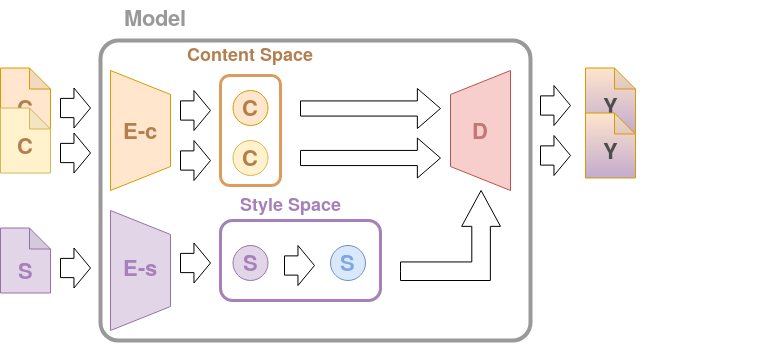
\includegraphics[scale=0.3]{pipelinemodel.png}
\end{figure}


\begin{itemize}
	\item \textcolor{blue}{\textbf{Content Encoder E-c}} and \textcolor{Plum}{\textbf{Style Encoder E-s}}
	\vspace{10pt}
	\item \textcolor{red}{\textbf{Random sampling}} from a Gaussian centered at \textcolor{Plum}{\textbf{style encoding}}
	\vspace{10pt}
\end{itemize}

\end{frame}

\begin{frame}
  \addtocounter{framenumber}{-1}
\frametitle{Our Approach - Content Loss}
\begin{figure}
\centering
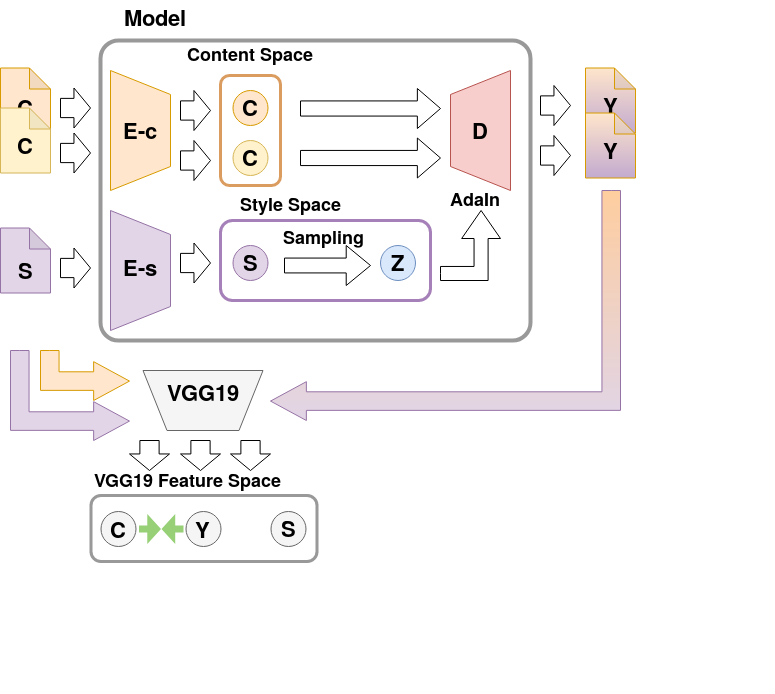
\includegraphics[scale=0.3]{pipelinecontent.png}
\end{figure}


\begin{itemize}
	\item \textcolor{blue}{\textbf{Content Loss}}: Perceptual loss using pretrained \textbf{VGG19} loss network
	\vspace{10pt}
\end{itemize}

\end{frame}

\begin{frame}
  \addtocounter{framenumber}{-1}
\frametitle{Our Approach - Style Loss}
\begin{figure}
\centering
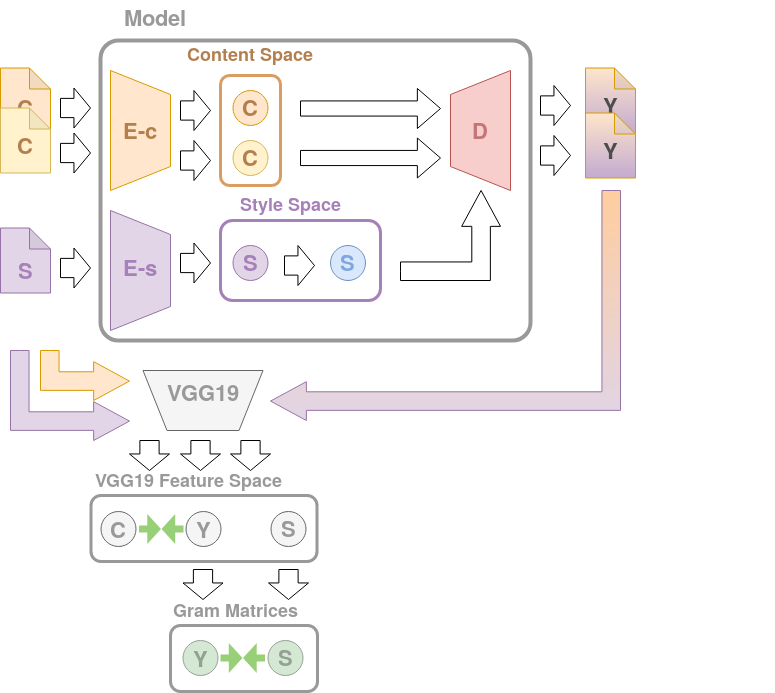
\includegraphics[scale=0.3]{pipelinestyle.png}
\end{figure}


\begin{itemize}
	\item \textcolor{Plum}{\textbf{Style Loss}}: Gram matrices of feature activations
	\vspace{10pt}
\end{itemize}

\end{frame}


\begin{frame}
  \addtocounter{framenumber}{-1}
\frametitle{Our Approach - Disentanglement Loss}
\begin{figure}
\centering
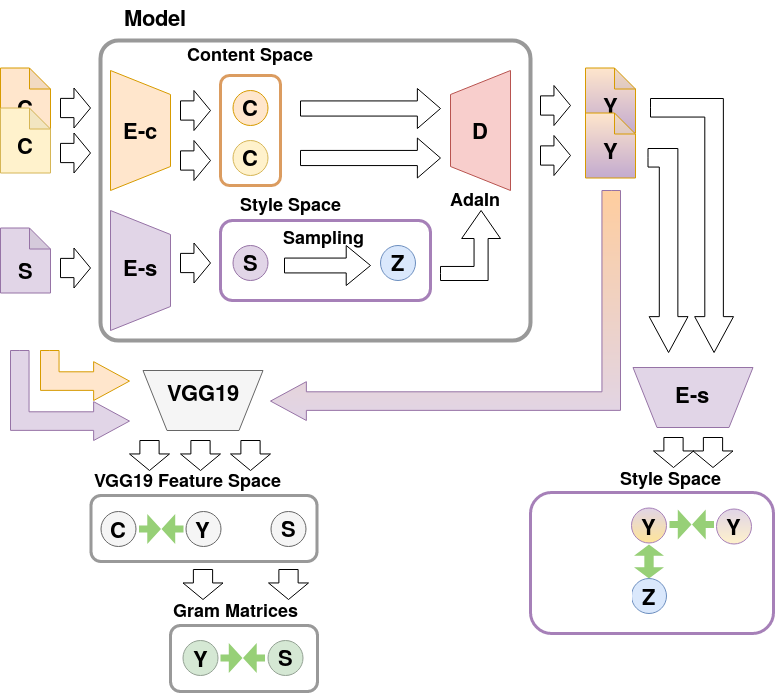
\includegraphics[scale=0.3]{pipelinedisentangled.png}
\end{figure}


\begin{itemize}
	\item \textcolor{Plum}{\textbf{Disentanglement Loss}}: Disentangles content and style
	\vspace{10pt}
\end{itemize}

\end{frame}
\begin{frame}
  \addtocounter{framenumber}{-1}
\frametitle{Our Approach - Regularization Loss}
\begin{figure}
\centering
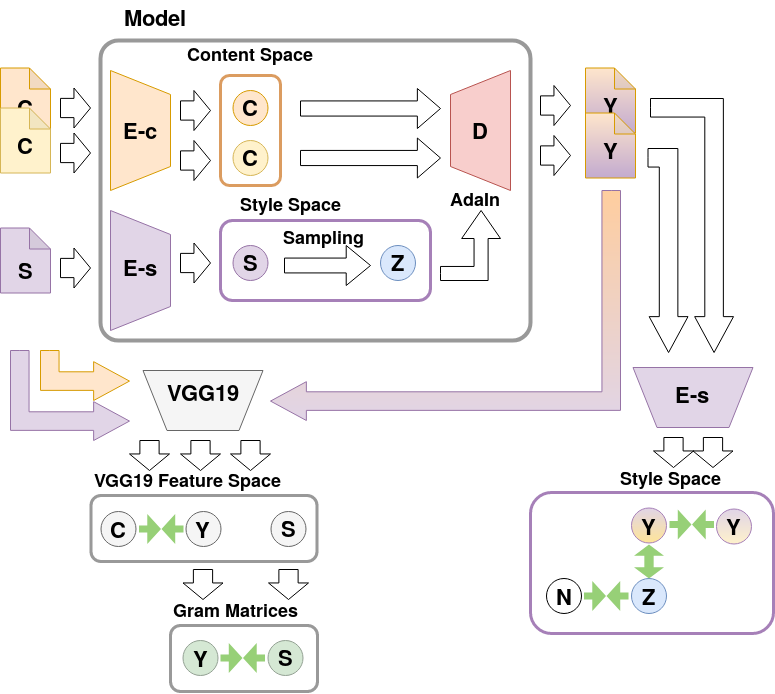
\includegraphics[scale=0.3]{pipelinefull.png}
\end{figure}


\begin{itemize}
	\item \textcolor{Plum}{\textbf{Regularization}}: Regularizes style distribution
	\vspace{10pt}
\end{itemize}

\end{frame}

\begin{frame}
  \addtocounter{framenumber}{-1}
\frametitle{Our Approach - Implementation Progress}
\begin{figure}
\centering
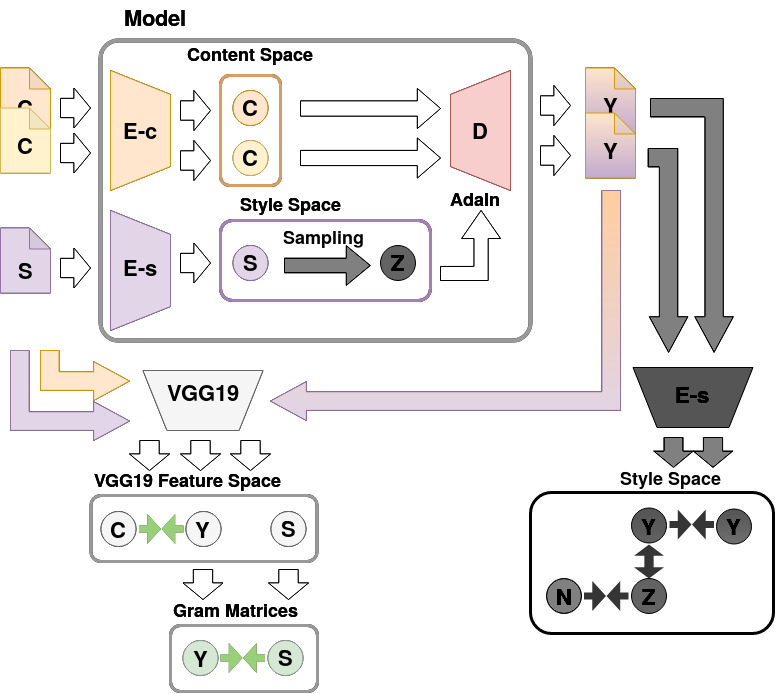
\includegraphics[scale=0.3]{pipelinecurrent.png}


\end{figure}
\centering
\textcolor{gray}{\textbf{Gray components are not yet implemented.}}

\end{frame}

\begin{frame}
\frametitle{Code}

Available implementations:
	\vspace{10pt}

\begin{itemize}
	\item \textcolor{red}{\textbf{Loss network}}: \textbf{torchvision}'s\footnote{\url{https://pytorch.org/docs/stable/torchvision/models.html}} pretrained VGG19
	\vspace{10pt}
	\item \textcolor{blue}{\textbf{Content}} and \textcolor{Plum}{\textbf{style}} losses and \textbf{AdaIn}: Unofficial implementation\footnote{https://github.com/naoto0804/pytorch-AdaIN} of \cite{adain}
	\vspace{10pt}
	\item \textcolor{blue}{\textbf{Perceptual}} and \textcolor{Plum}{\textbf{style}} losses pytorch implementation\footnote{\url{https://github.com/leongatys/PytorchNeuralStyleTransfer}} of \cite{gatys}
\end{itemize}
	\vspace{10pt}

Unfortunately, for \cite{disentanglement}, \textbf{\textcolor{red}{no implementation is available}} so far.


\end{frame}

\begin{frame}
\frametitle{Datasets}

\textcolor{blue}{\textbf{Content images}}: Places365\footnote{\url{http://places2.csail.mit.edu/download.html}} dataset with different sceneries

\begin{multicols*}{3}

\begin{figure}
	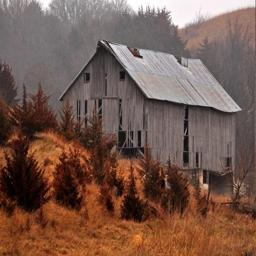
\includegraphics[width=0.5\linewidth]{places0.jpg}
\end{figure}

\columnbreak

\begin{figure}
	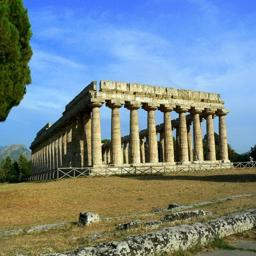
\includegraphics[width=0.5 \linewidth]{places1.jpg}
\end{figure}

\columnbreak

\begin{figure}
	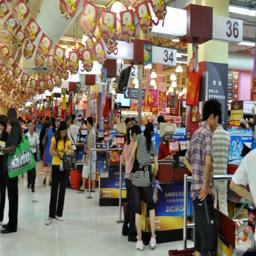
\includegraphics[width=0.5\linewidth]{places2.jpg}
\end{figure}

\end{multicols*}



\textcolor{Plum}{\textbf{Style images}}: WikiArt\footnote{\url{https://github.com/cs-chan/ArtGAN}} contains artistic images


\begin{multicols*}{3}

\begin{figure}
	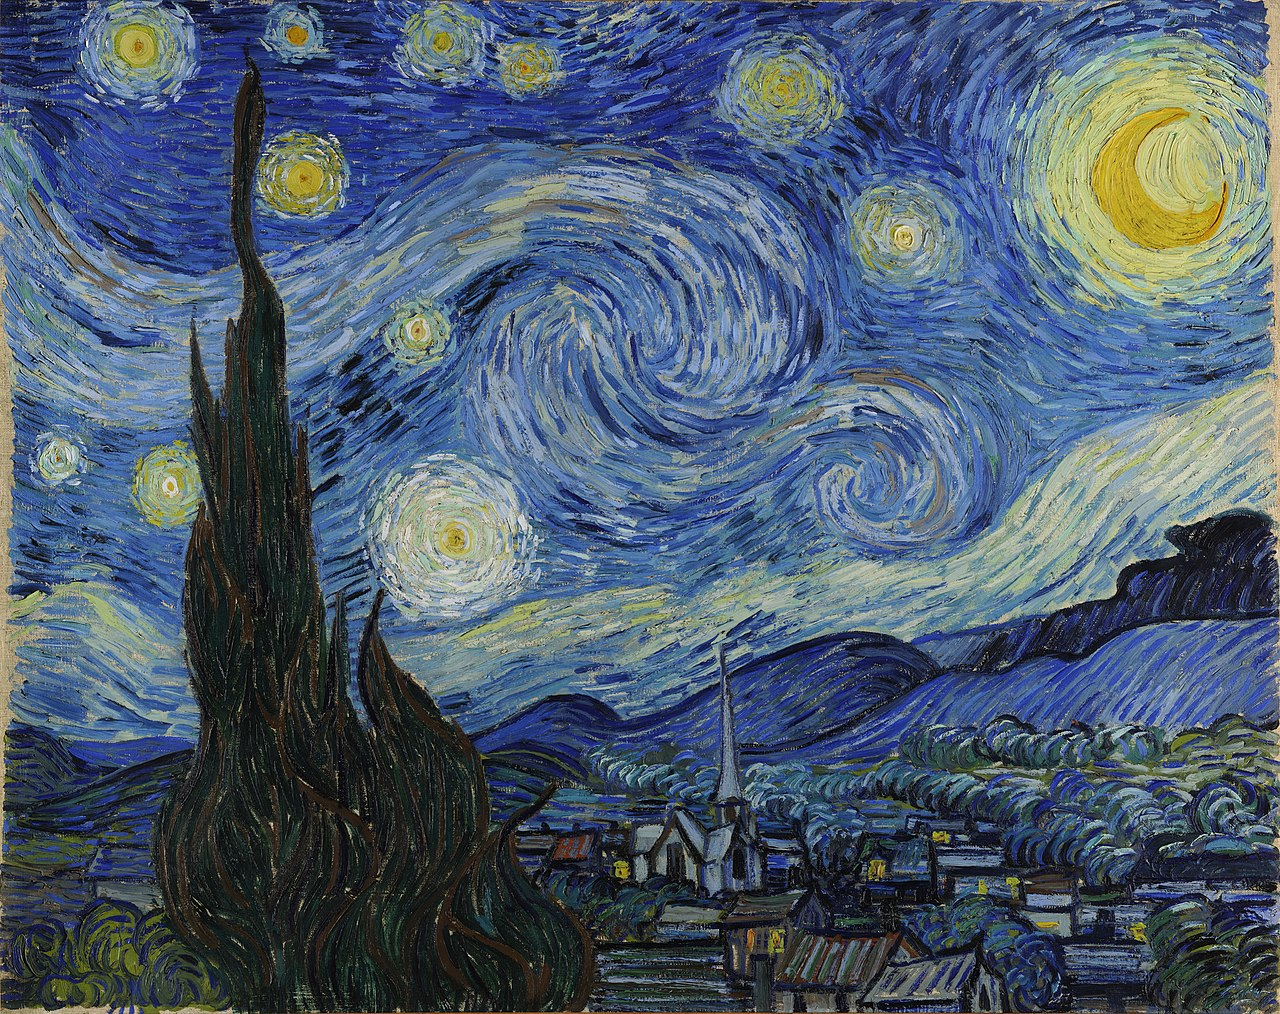
\includegraphics[width=0.6\linewidth]{starry_night.jpg}
\end{figure}

\columnbreak

\begin{figure}
	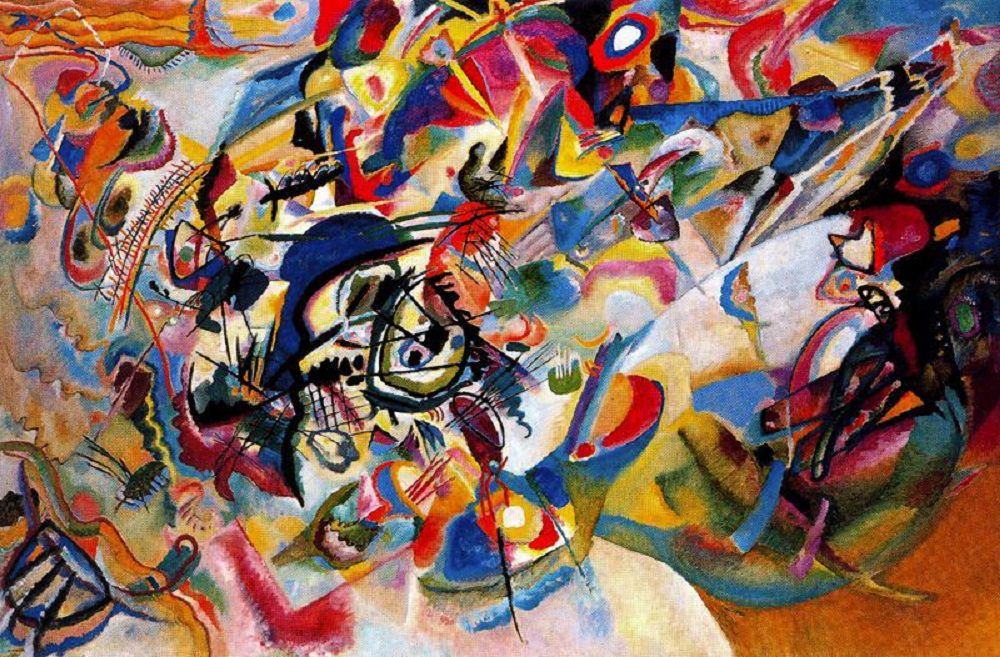
\includegraphics[width=0.6 \linewidth]{kandinsky_composition.jpg}
\end{figure}

\columnbreak

\begin{figure}
	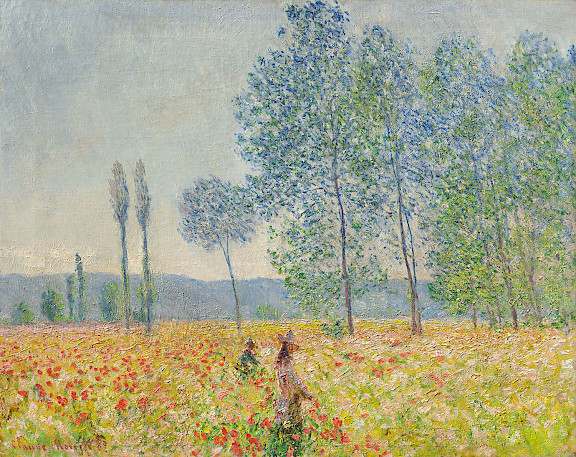
\includegraphics[width=0.6\linewidth]{monet.jpg}
\end{figure}

\end{multicols*}


Lack of large GPU resources: $\rightarrow$ \textcolor{red}{\textbf{downsample}} images to a \textbf{64x64} resolution and only \textcolor{red}{\textbf{shallow}} networks.

\end{frame}

\begin{frame}
\frametitle{Evaluation}

To our best knowledge there is \textcolor{red}{\textbf{no data-driven metric}} to asses the quality of stylizations.

\vspace{10pt}

Common subjective assessment methods:

\begin{itemize}
	\item \textcolor{blue}{\textbf{Preference Rate}}: Probands \textbf{select most appealing} result among different stylizations
	\item \textcolor{blue}{\textbf{Deception Rate}}: Probands try to \textbf{identify a real artistic image} mixed between stylizations
\end{itemize}

\vspace{10pt}

We focus on \textbf{\textcolor{red}{interpolations between multiple styles}}!

\vspace{10pt}

\textcolor{Plum}{\textbf{We would be glad if course participants and / or chair members could participate!}}


\end{frame}

\begin{frame}
\frametitle{First Results}

\begin{center}
\textcolor{blue}{\textbf{content image}} \hspace{0.5cm}  \textcolor{Plum}{\textbf{style image}} \hspace{0.75cm} \textbf{Stylization}

\begin{figure}
	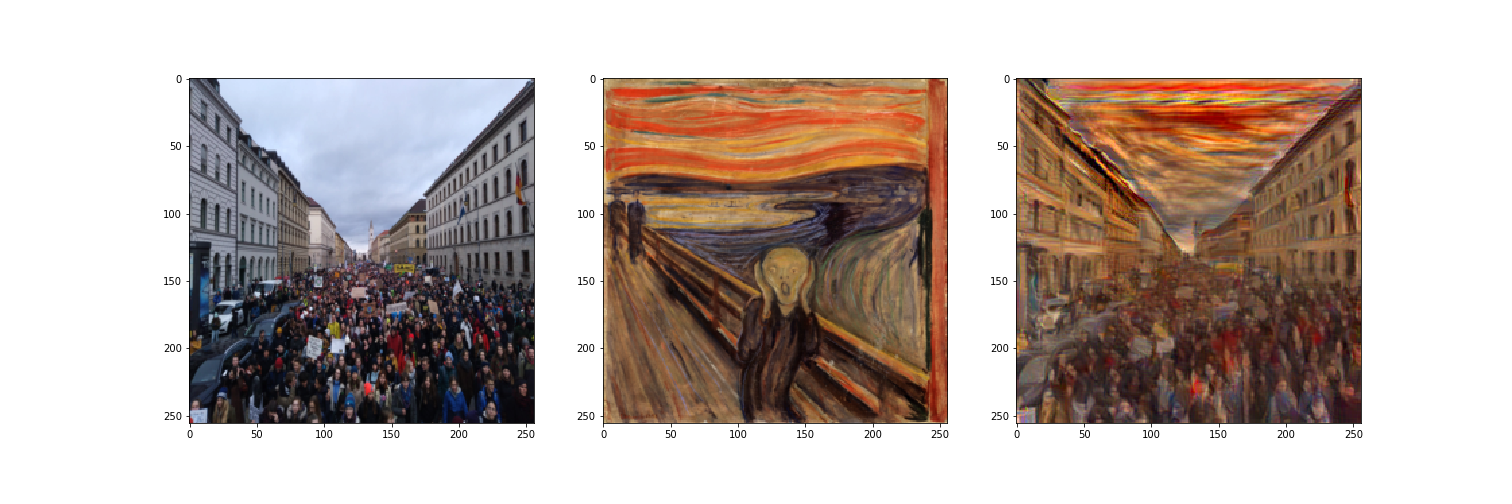
\includegraphics[width=1.0\linewidth]{scream_adain_3001.png}
\end{figure}

\vspace{-1cm}

\begin{figure}
	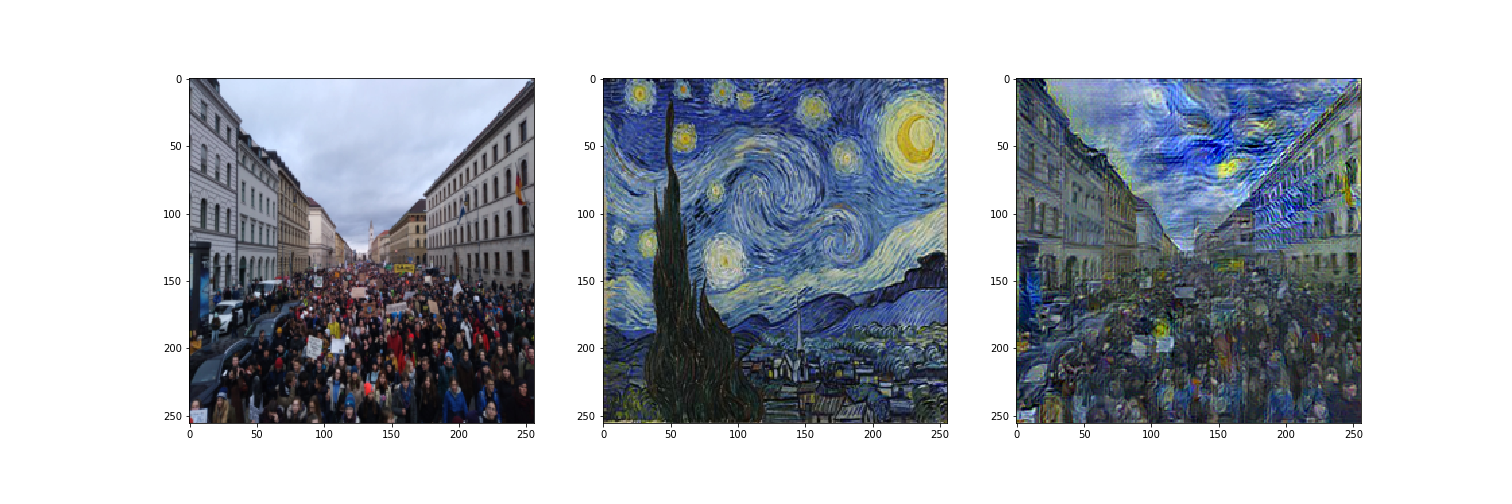
\includegraphics[width=1.0\linewidth]{starry_night_relu4_1e-2_lr1e-4.png}
\end{figure}

\end{center}

\end{frame}

\begin{frame}
\frametitle{Milestones}

What we want to achieve until the next presentation:
	\vspace{10pt}
\begin{itemize}
	\item Get the \textcolor{Plum}{\textbf{style transfer}} working
	\vspace{10pt}
	\item Implement the \textcolor{Plum}{\textbf{disentanglement loss}}
	\vspace{10pt}
	\item Implement \textcolor{red}{\textbf{sampling}} from a latent style distribution
	\vspace{10pt}
	\item Fine-tune the architecture and train a final evaluation-ready model
	\vspace{10pt}
	\item (Possibly) set up a \textcolor{blue}{\textbf{survey}} and \textcolor{blue}{\textbf{participants}} for our evaluation
	\\
	This includes getting \textbf{baselines} running as well
\end{itemize}
\end{frame}

\begin{frame}
\frametitle{Baselines}

Possible baselines for evaluation on \textcolor{blue}{\textbf{preference rate}} include:
	\vspace{10pt}

\begin{itemize}
\item The original style transfer paper \cite{gatys}
	\vspace{10pt}
	\item The \textbf{AdaIn} paper \cite{adain}: Same decoder for \textbf{\textcolor{blue}{content}} and \textcolor{Plum}{\textbf{style}}
	\vspace{10pt} 
	\item Learning a \textbf{linear transformation} on an image embedding for style transfer \cite{linear}
	\vspace{10pt} 
	
\end{itemize}

Possibly problematic may be \textcolor{red}{\textbf{model sizes}} and \textcolor{red}{\textbf{computation times}} due to our limited resources.


\end{frame}

\begin{frame}[allowframebreaks]
        \frametitle{References}


        \printbibliography
\end{frame}

\begin{frame}
	\frametitle{Perceptual Loss}
	
Instead of a pixel-wise loss between input and output: \\
$\rightarrow$ \textbf{\textcolor{blue}{error between feature activations}} of layer(s) $i$ provided by a pre-trained model $\Phi$
\vspace{10pt}

\begin{equation*}
	\mathcal{L}_{\Phi}(y, \hat{y}) = \frac{1}{C_i \times H_i \times W_i} \sum_i\lVert f^i_{\Phi}(y) - f^i_{\Phi}(\hat{y}) \rVert^2_2
\end{equation*}
\vspace{10pt}

Where $f^i$ are the \textbf{activation maps} of layer $i$ with a dimensionality of $C_i \times H_i \times W_i$.
\vspace{10pt}

Penalizes \textcolor{red}{\textbf{semantic discrepancies}} between $y$ and $\hat{y}$ (e.g. objects, composition, etc.)

\end{frame}

\begin{frame}
	\frametitle{Style Loss}

\textbf{\textcolor{Plum}{Gram matrices}} $G_i$ of feature activation maps  $f_i$ capture \textbf{\textcolor{red}{correlations between channels}}:

\begin{equation*}
	G_i(y) = \tilde{f}_{\Phi}^i(y) \tilde{f}_{\Phi}^i(y)^T
\end{equation*}

Where $\tilde{f}^i_{\Phi}$ are \textbf{flattened feature activation maps} of shape $C_i \times (H_i W_i)$.
\vspace{10pt}

$G_i(y)(c_1, c_2)$ captures how \textcolor{red}{\textbf{strongly correlated}} the features $c_1$ and $c_2$ are in the activation map $f_i$.

\vspace{10pt}	
	
The \textbf{\textcolor{Plum}{style loss}} is given as the \textbf{\textcolor{blue}{error between Gram matrices of feature maps}}:

\begin{equation*}
	\mathcal{L}_{\Phi}(y, \hat{y}) = \sum_i \frac{1}{C_i^2} \lVert G_i(y) - G_i(\hat{y}) \rVert^2_2
\end{equation*}
	
\end{frame}

\begin{frame}
\frametitle{Adaptive Instance Normalization}

\textbf{\textcolor{blue}{Instance Normalization}} is related to \textbf{Batch Normalization} but calculates \textbf{\textcolor{red}{instance-wise}} mean $\mu$ and variance $\sigma^2$, instead of using batch-wise statistics.

\vspace{10pt}

\cite{adain} showed that $\mu$ and $\sigma$ \textbf{\textcolor{Plum}{encapsulate style information}}:
\vspace{10pt}
$\rightarrow$ \textbf{Adaptive Instance Normalization}:
\begin{equation*}
	\text{AdaIn}(x, y) = \sigma(y) \frac{x - \mu(x)}{\sigma(x)} + \mu(y)
\end{equation*}
\vspace{10pt}

\textbf{\textcolor{red}{transfers instance-wise statistics}} from $y$ to $x$

\vspace{10pt}

\textbf{No learnable parameters!}

\end{frame}

\begin{frame}[allowframebreaks]
\frametitle{Variational Autoencoders}

\textbf{Autoencoders} encode an input $X$ to a latent space representation $z$ and try to reconstruct $X$ using only $z$. \\
$\rightarrow$ \textbf{\textcolor{red}{neglects variations in input distribution}} (e.g. noise) \\
$\rightarrow$ Latent space \textcolor{red}{\textbf{may not be smooth}}

\vspace{10pt}

\textbf{\textcolor{blue}{Variational Autoencoders}} sample $s$ from a \textbf{\textcolor{blue}{distribution parametrized by $z$}} (usually Gaussian) instead

\begin{figure}
\centering
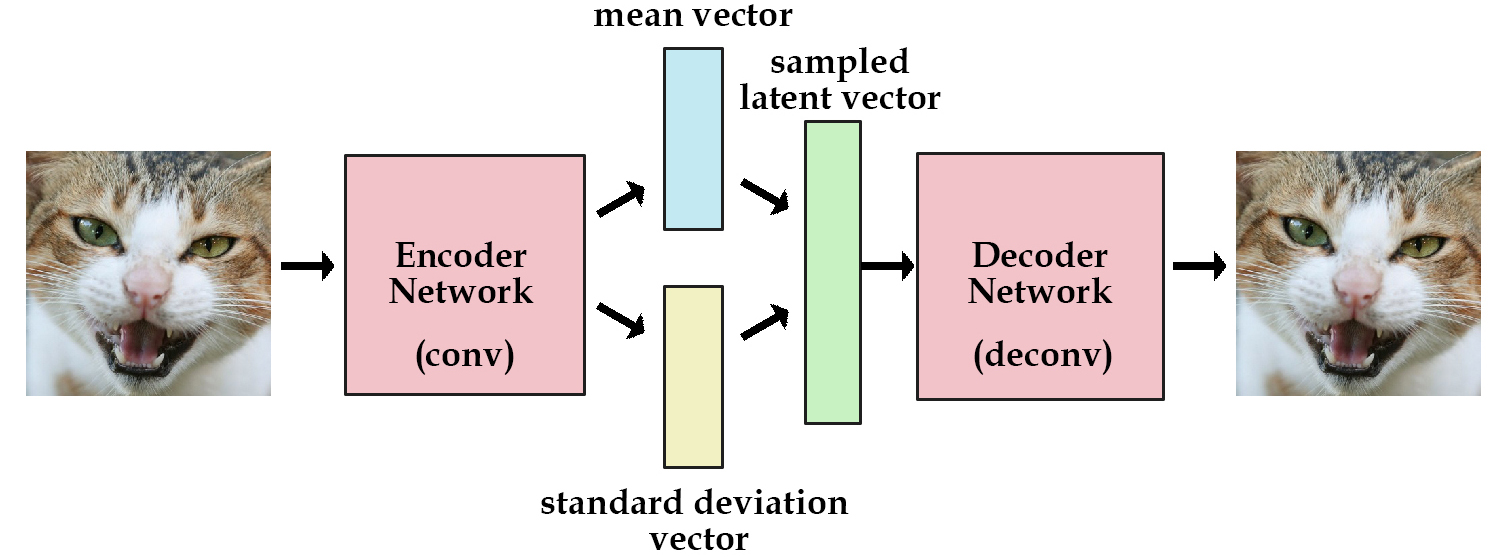
\includegraphics[scale=0.15]{vae.jpg}
\caption{taken from \url{http://kvfrans.com/variational-autoencoders-explained/}}
\end{figure}

To enforce a \textcolor{Plum}{\textbf{smooth latent space}} the learned distribution is \textbf{\textcolor{blue}{regularized}} using the KL-divergence:
\vspace{10pt}

\begin{equation*}
	\mathcal{L} = \mathbb{KL}(q_{\text{enc}}(s | X) \Vert p(z))
\end{equation*}
\vspace{10pt}

Where $q_{\text{enc}}(s | X)$ describes the distribution of latent representations $s$ given an input $X$ and $p(z)$ is set to be a standard normal distribution.
\\

\vspace{10pt}
$\rightarrow$ forces \textbf{\textcolor{blue}{latent distribution}} to be \textbf{\textcolor{red}{close to a standard normal distribution}}.


\end{frame}

\end{document}